\documentclass[fleqn,10pt]{wlscirep}
\usepackage[utf8]{inputenc}
\usepackage[T1]{fontenc}
\usepackage{graphicx}

%=================================================================
%  Revision Markup Commands
%=================================================================
\newcommand{\revtag}[2]{[\textbf{R#1-C#2}]}
\newcommand{\Rone}[1]{\textcolor{red}{#1}}
\newcommand{\Rtwo}[1]{\textcolor{blue}{#1}}

\renewcommand{\figurename}{Supplementary Figure}
\renewcommand{\thefigure}{S\arabic{figure}}

\renewcommand{\tablename}{Supplementary Table}
\renewcommand{\thetable}{S\arabic{table}}

\begin{document}

\section*{Appendix A}

\setcounter{figure}{0} % Reset figure counter to start at S1 for the appendix
\setcounter{table}{0} % Reset table counter to start at S1 for the appendix

\begin{figure}[!htbp]
\centering
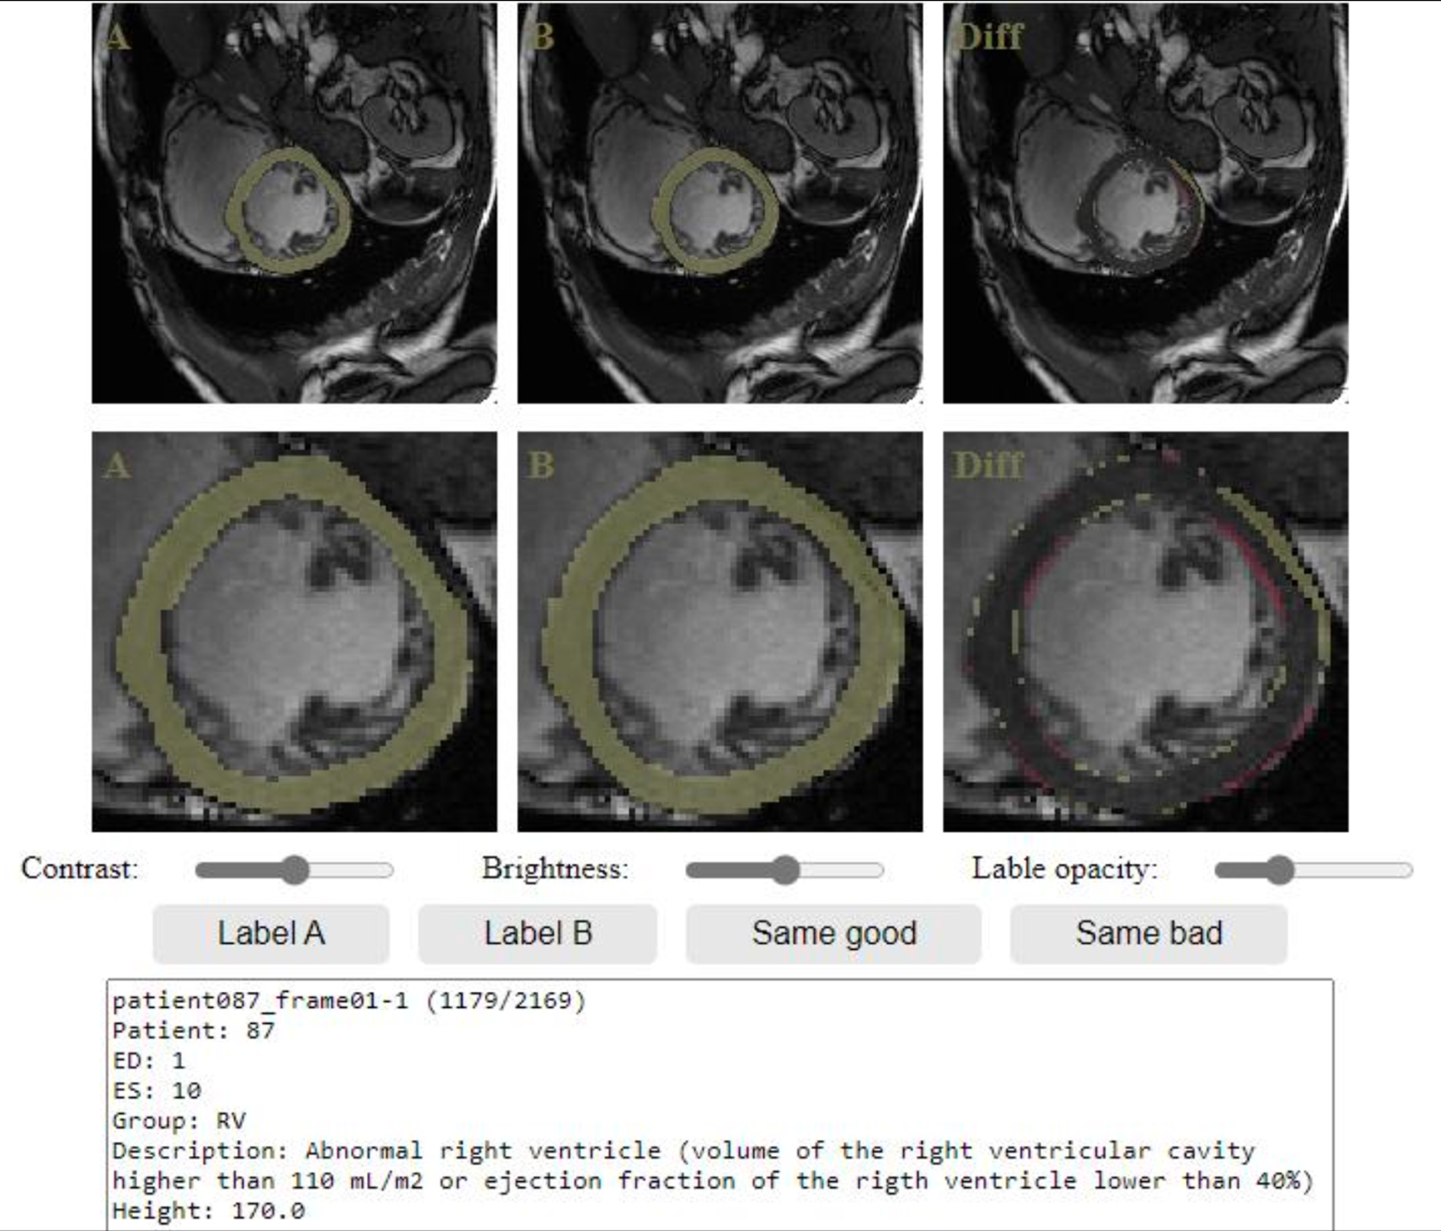
\includegraphics[width=0.8\linewidth]{img/56_fig_s1_interface.png}
\caption{The user interface of the custom software application developed for expert validation of segmentation masks. The interface allows a side-by-side comparison of two anonymized masks (Mask A and Mask B) overlaid on the cardiac MRI scan. The validating clinician can adjust image brightness and contrast, control mask opacity, and zoom in on specific regions. Based on this detailed visual analysis, the expert selects one of four options to grade the relative accuracy of the masks, ensuring an objective and thorough evaluation process.}
\label{fig:validation_app}
\end{figure}

\begin{figure}[!htbp]
\centering
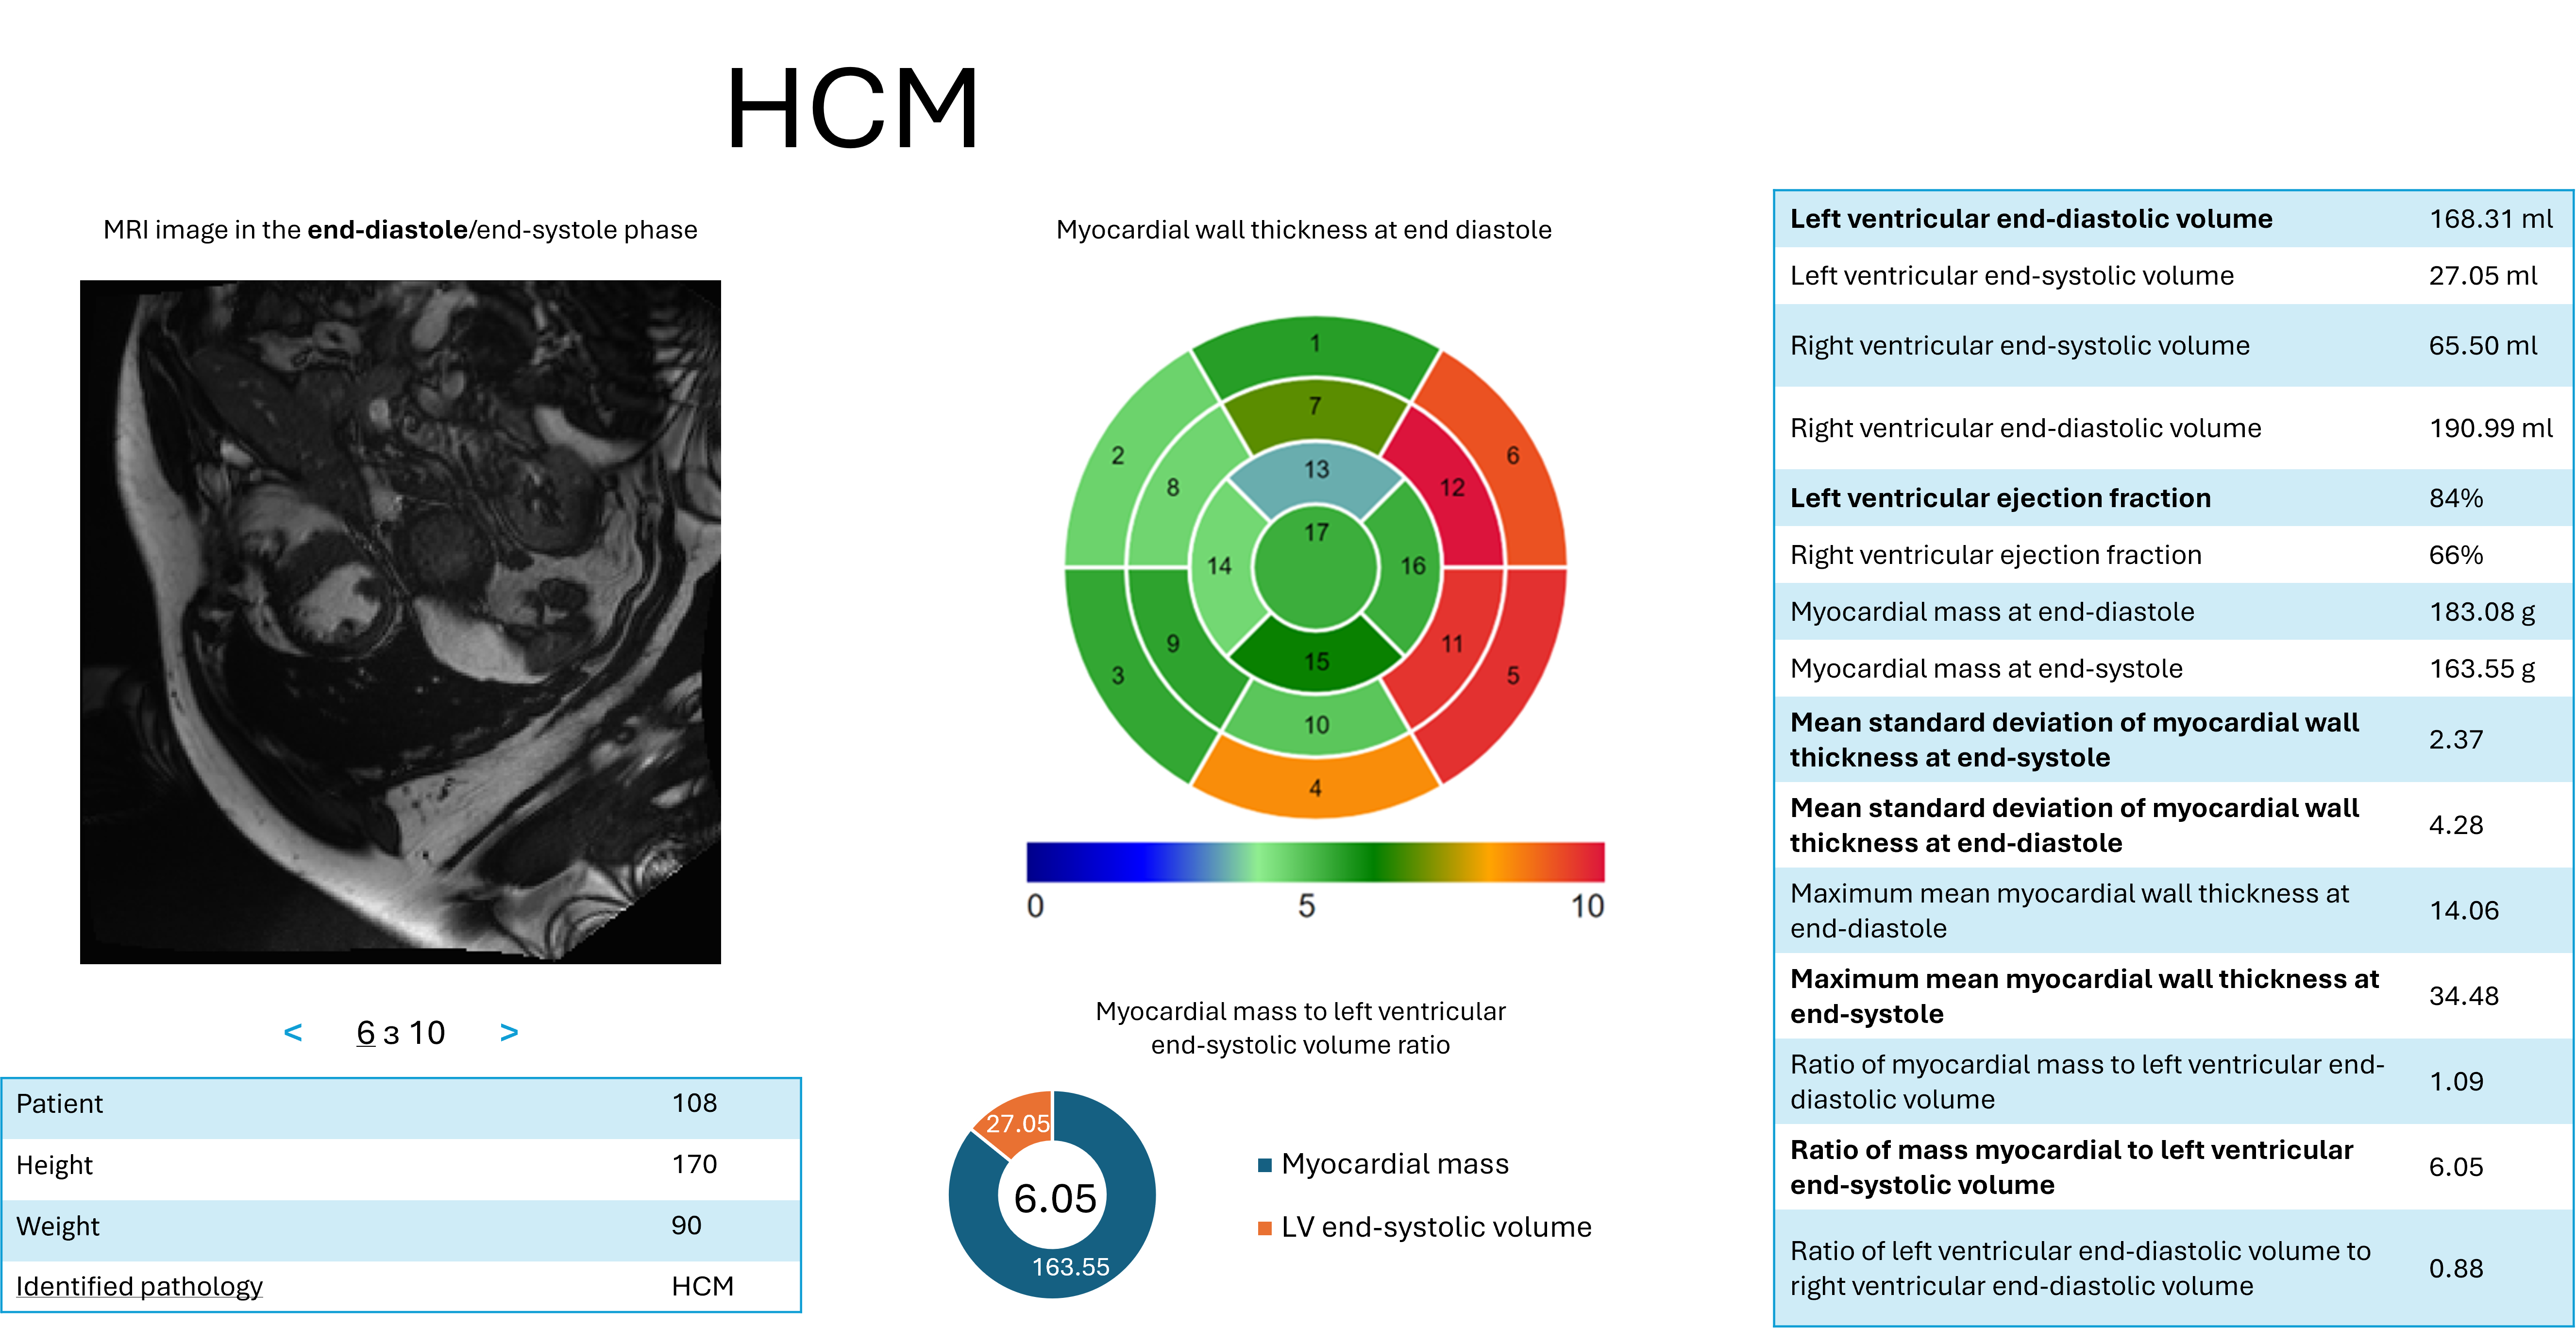
\includegraphics[width=1.0\linewidth]{img/56_fig_s2_HCM.png}
\caption{Visualization of HCM, illustrating thickened myocardial segments and high ejection fraction.}
\label{fig:hcm_visualization}
\end{figure}

\begin{figure}[!htbp]
\centering
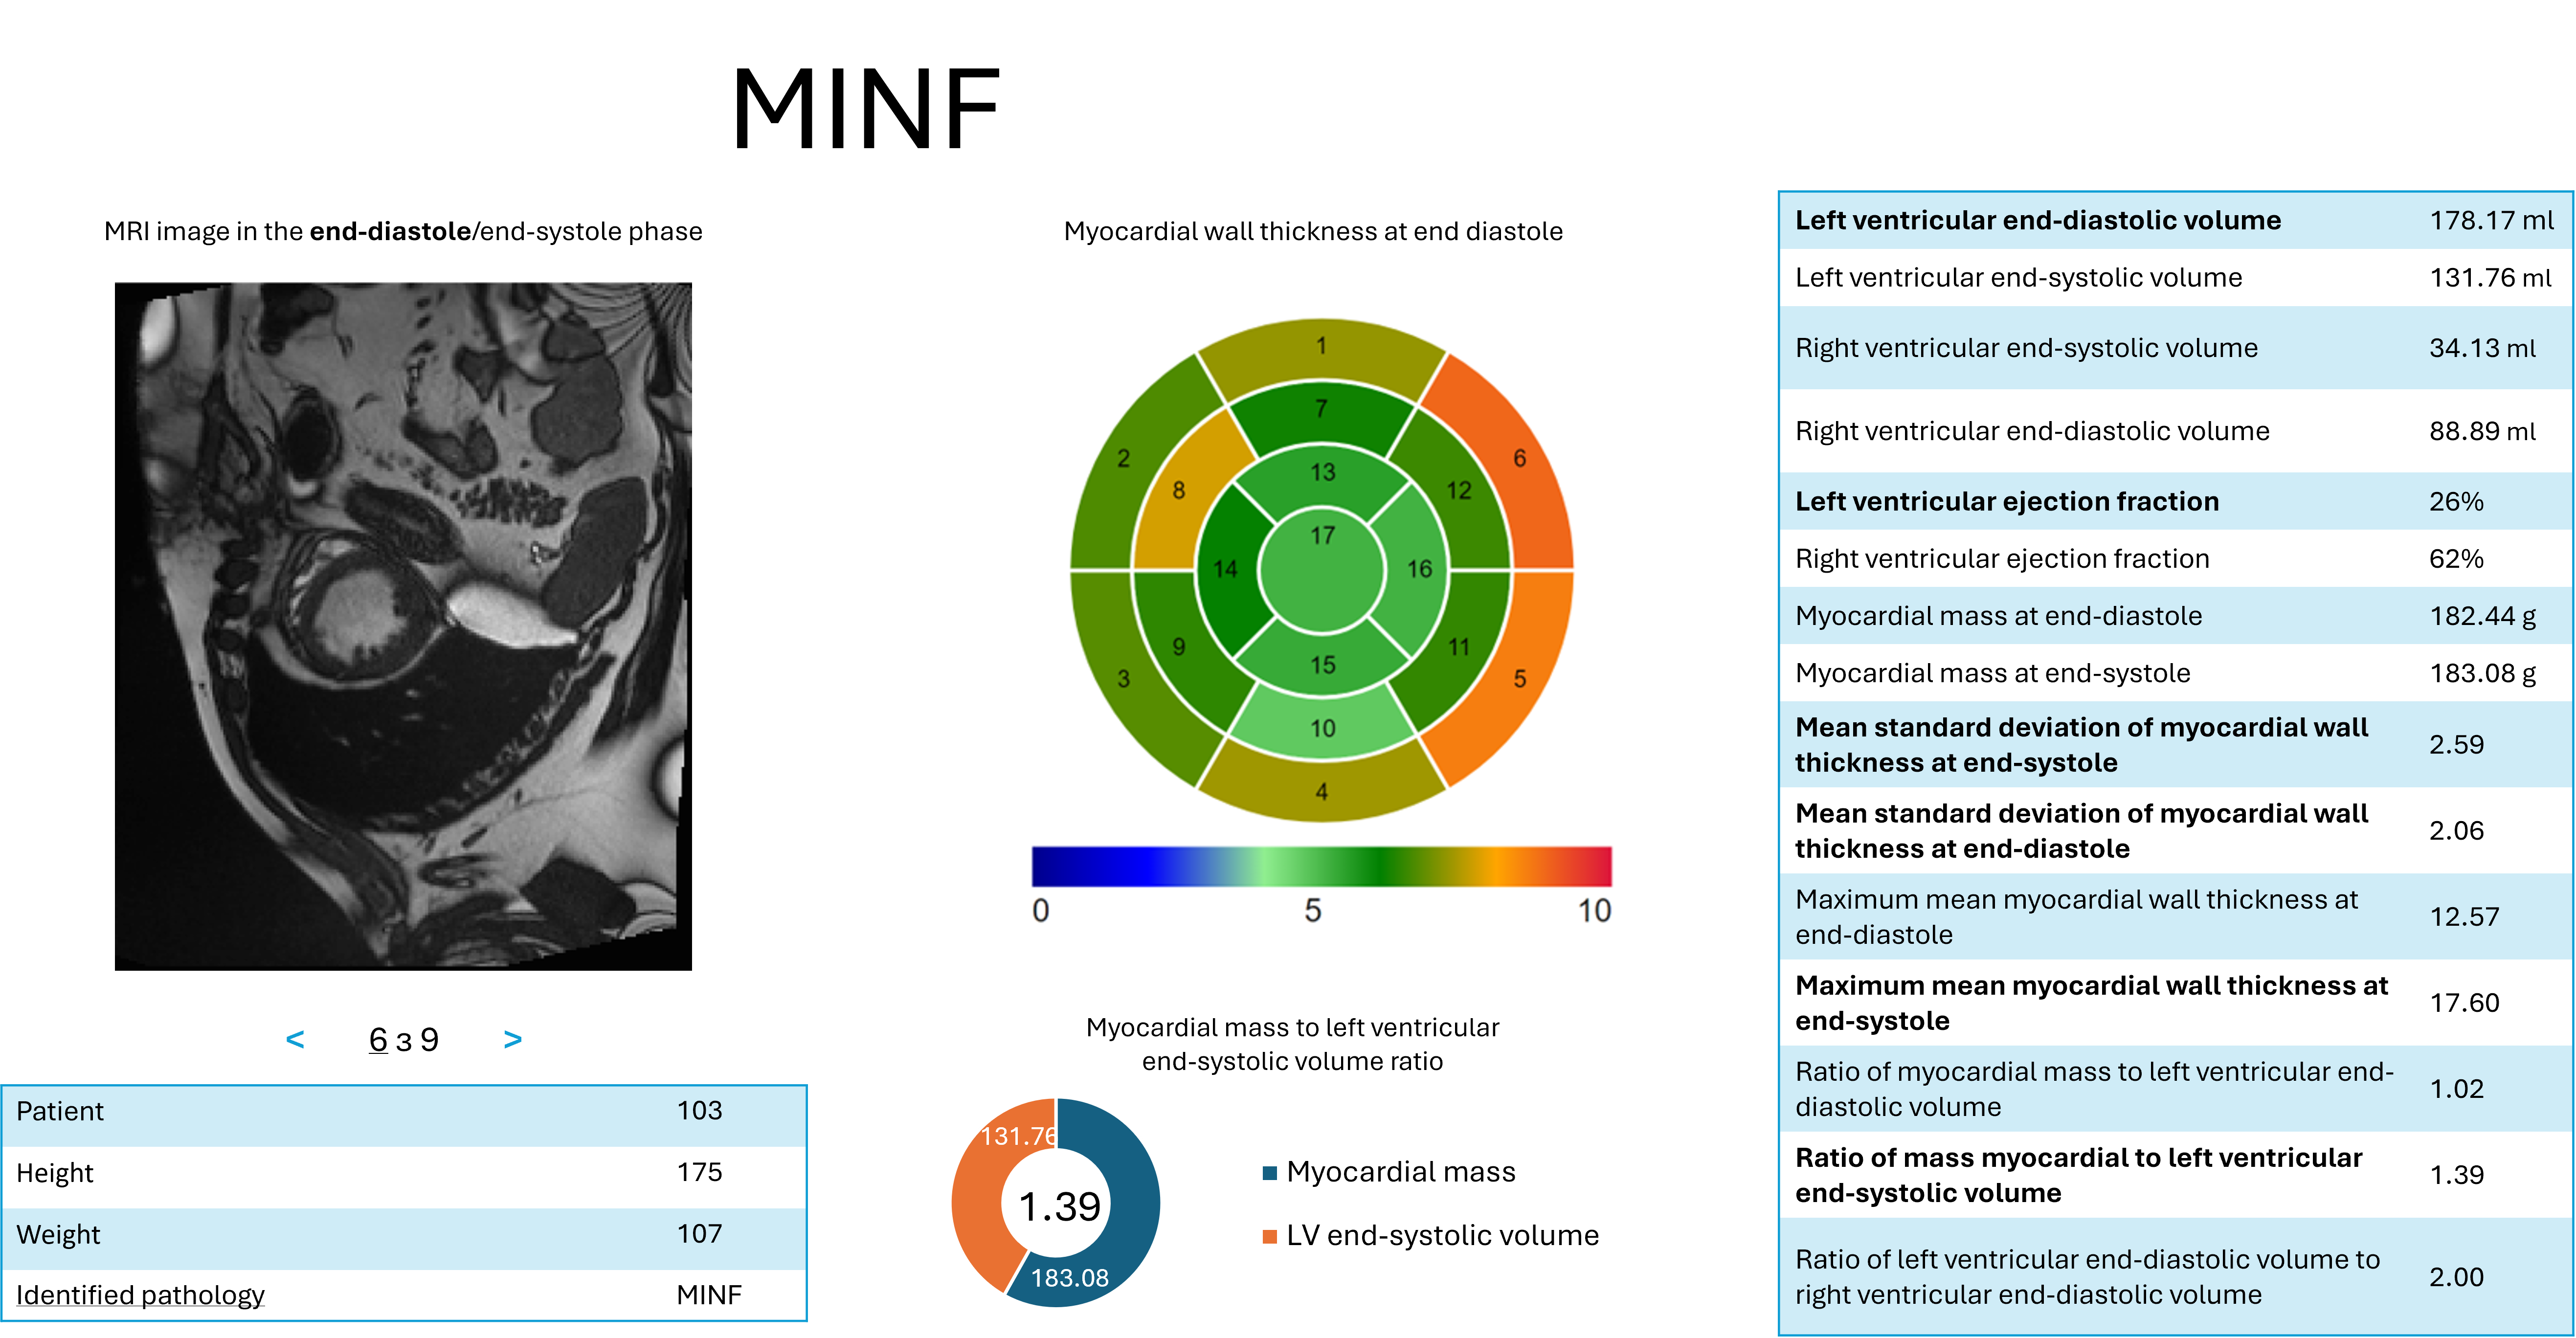
\includegraphics[width=1.0\linewidth]{img/56_fig_s3_MINF.png}
\caption{Visualization of MINF, highlighting reduced ejection fraction and irregular myocardium thickness.}
\label{fig:minf_visualization}
\end{figure}

\begin{figure}[!htbp]
\centering
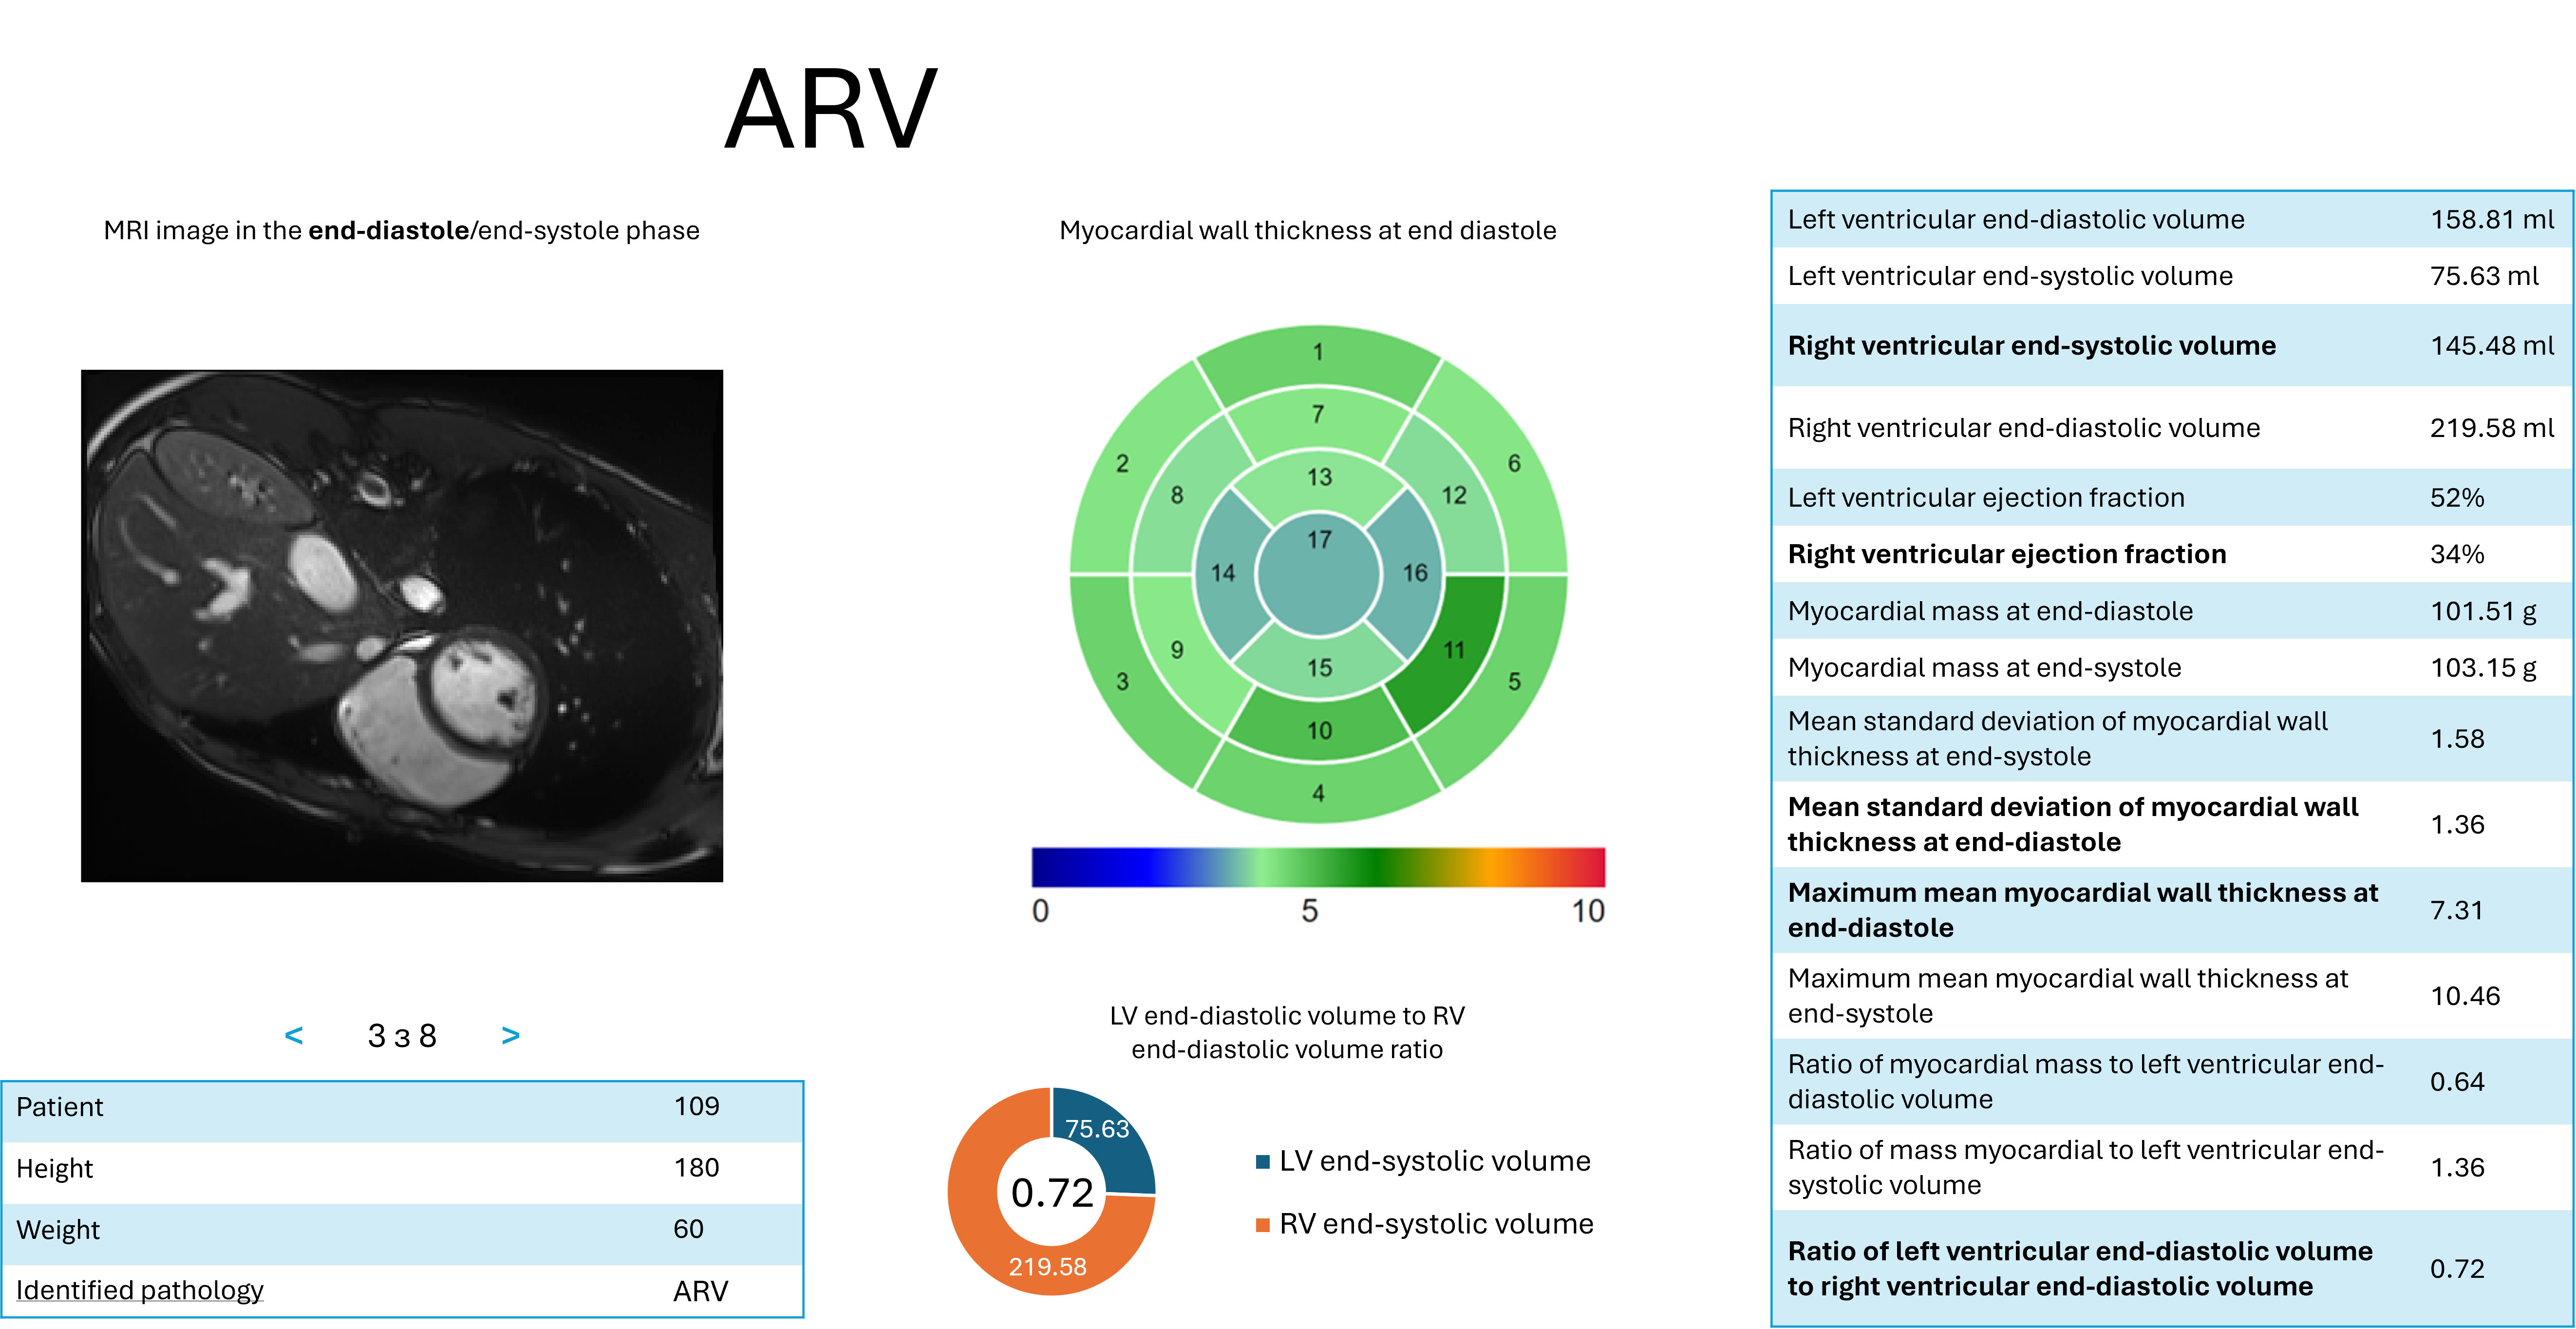
\includegraphics[width=1.0\linewidth]{img/56_fig_s4_ARV.png}
\caption{Visualization of ARV, illustrating enlarged RV and weakened systolic performance.}
\label{fig:arv_visualization}
\end{figure}

\begin{figure}[!htbp]
\centering
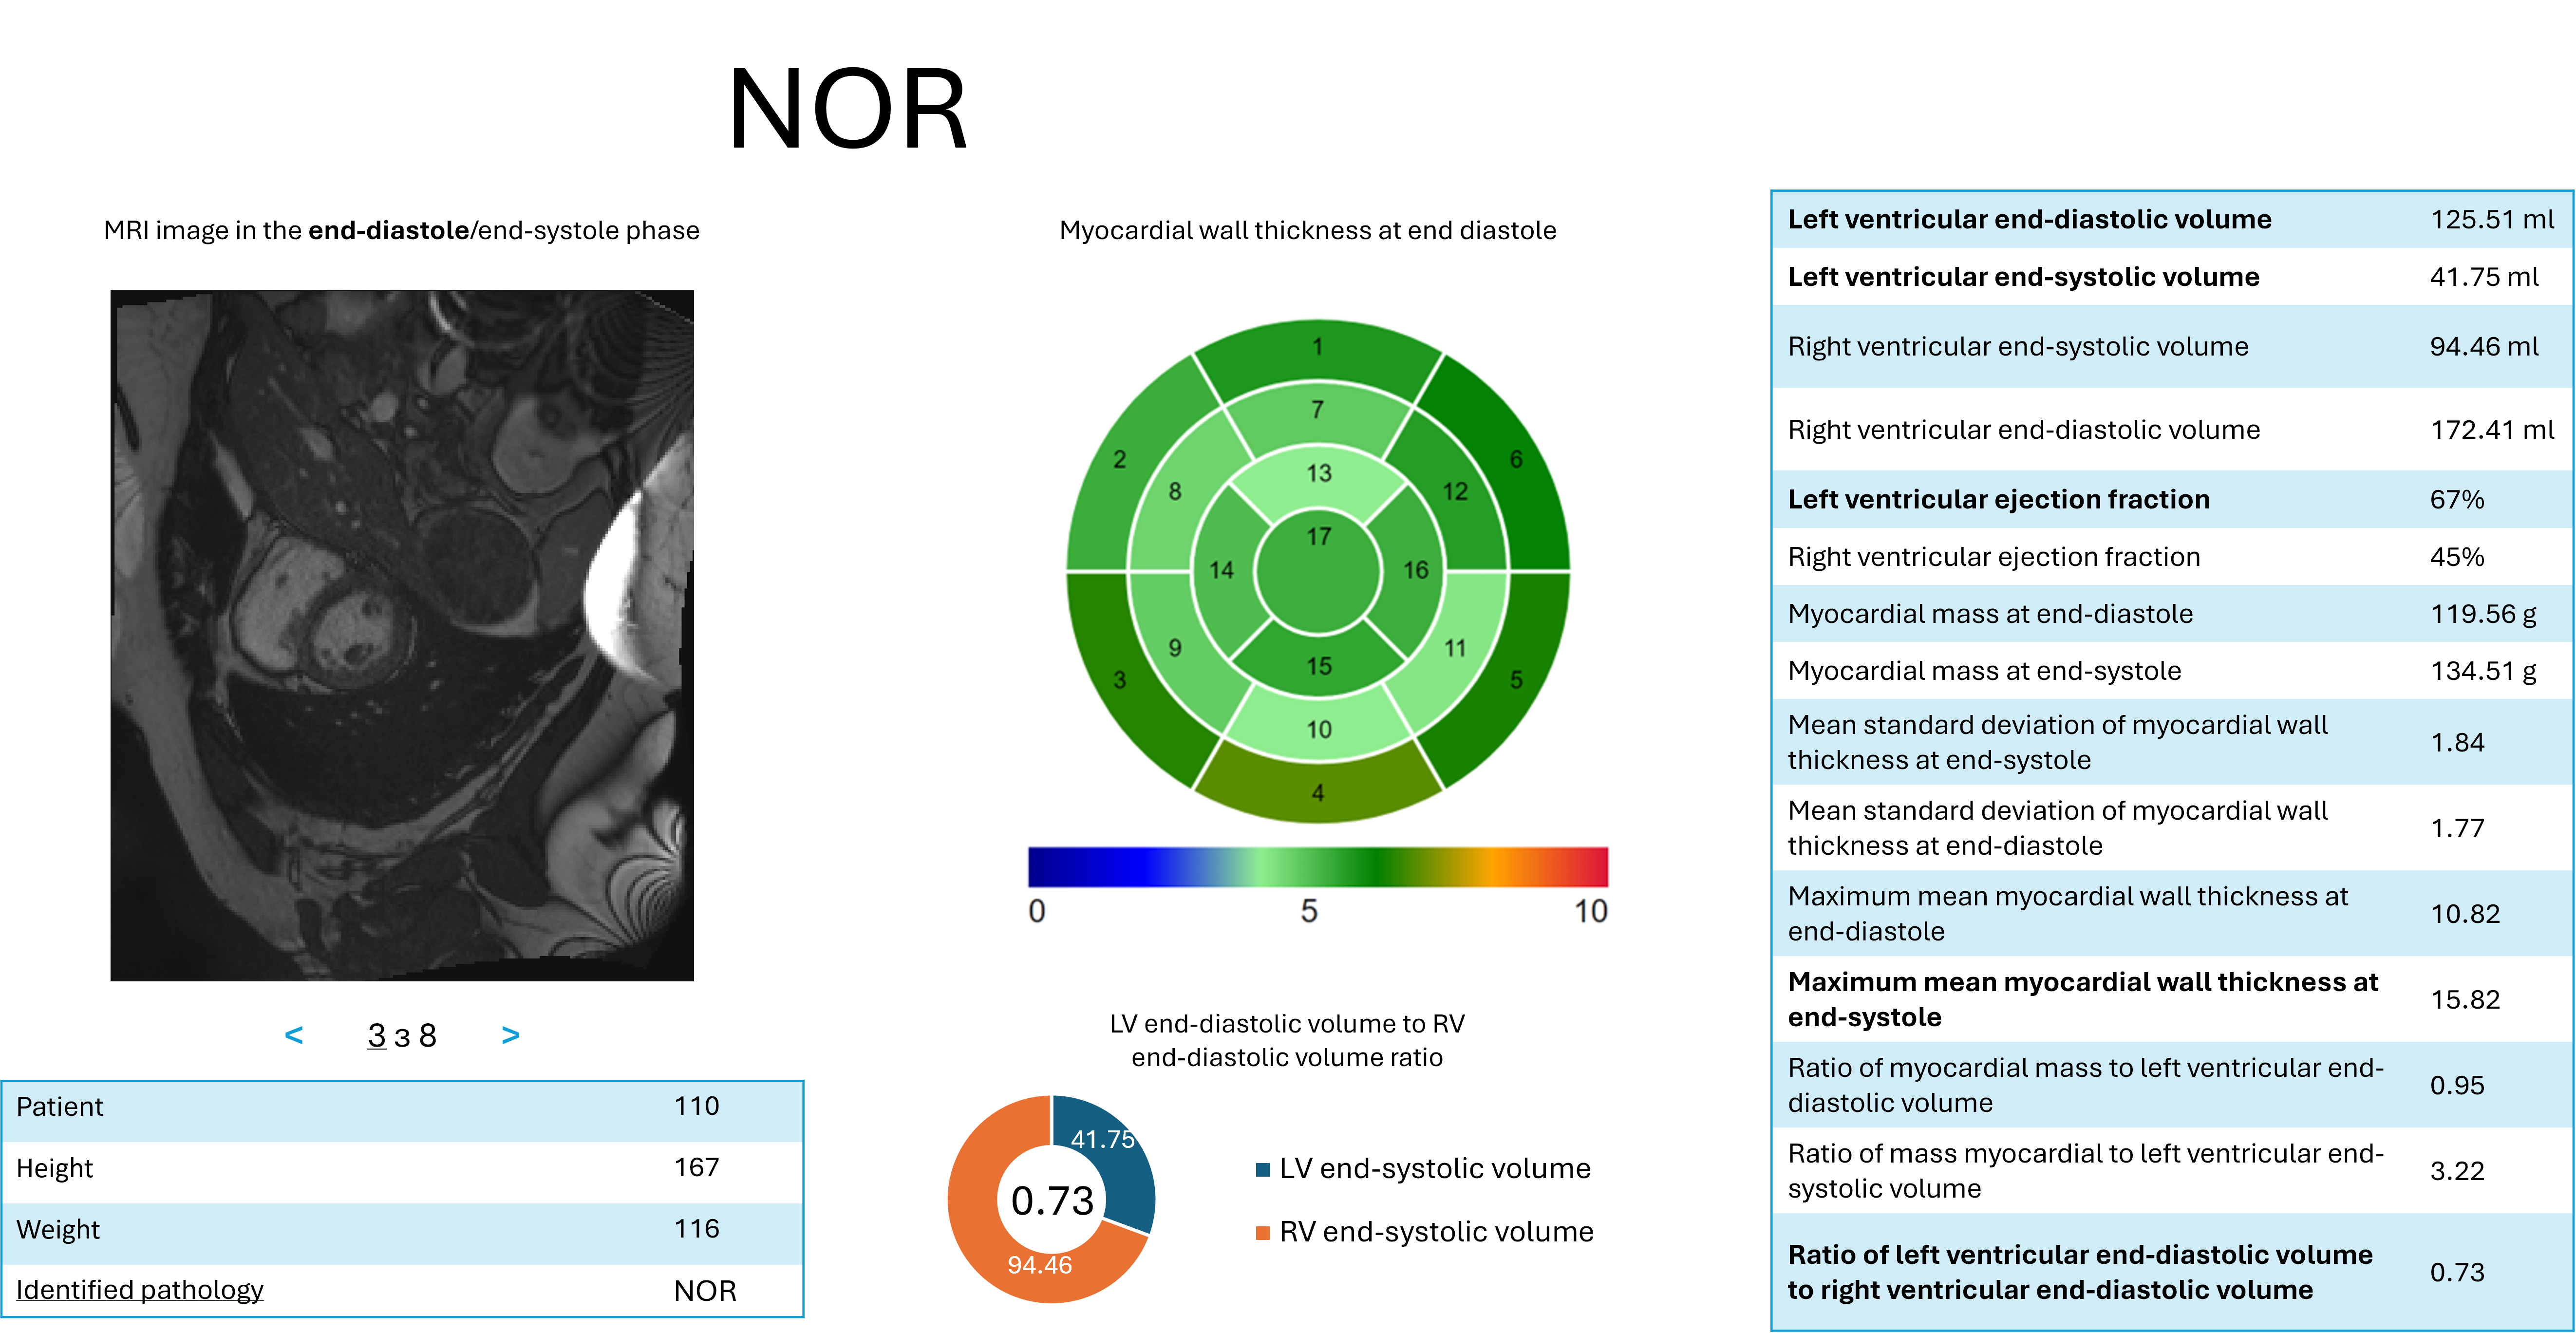
\includegraphics[width=1.0\linewidth]{img/56_fig_s5_NOR.png}
\caption{Visualization of NOR, emphasizing balanced ventricular volumes and normal contractility.}
\label{fig:nor_visualization}
\end{figure}

\begin{table}[ht]
  \centering
  \caption{\Rtwo{\revtag{2}{1}Detailed segmentation performance on the M\&Ms dataset by scanner vendor and model. Dice scores are reported for each cardiac structure and phase. The baseline performance on the ACDC training-domain scanners is highlighted in bold for reference. The results illustrate a performance gradient, with scanners most similar to the ACDC domain (Philips 1.5T, other Siemens 1.5T) performing best, and those with significant technical differences (GE scanners) showing a marked drop in accuracy.}}
  \label{tab:mms_breakdown}
  \begin{tabular}{lcccccc}
    \toprule
    \textbf{Scanner Vendor and Model (Field Strength)} & \textbf{LV-ED} & \textbf{LV-ES} & \textbf{RV-ED} & \textbf{RV-ES} & \textbf{MYO-ED} & \textbf{MYO-ES} \\
    \midrule
    \textbf{Siemens Area/Trio Tim (1.5T/3.0T) [ACDC]} & \textbf{0.974} & \textbf{0.940} & \textbf{0.947} & \textbf{0.915} & \textbf{0.896} & \textbf{0.920} \\
    \midrule
    \multicolumn{7}{l}{\textit{M\&Ms Dataset Scanners}} \\
    Philips Medical Systems, Achieva (1.5T) & 0.951 & 0.911 & 0.936 & 0.893 & 0.840 & 0.879 \\
    SIEMENS, Symphony (1.5T) & 0.947 & 0.922 & 0.882 & 0.825 & 0.816 & 0.863 \\
    SIEMENS, Avanto (1.5T) & 0.945 & 0.927 & 0.894 & 0.873 & 0.821 & 0.871 \\
    SIEMENS, SymphonyTim (1.5T) & 0.927 & 0.926 & 0.907 & 0.867 & 0.753 & 0.831 \\
    SIEMENS, Avanto Fit (1.5T) & 0.916 & 0.924 & 0.902 & 0.880 & 0.752 & 0.843 \\
    GE MEDICAL SYSTEMS, Signa Explorer (1.5T) & 0.859 & 0.896 & 0.898 & 0.887 & 0.689 & 0.805 \\
    GE MEDICAL SYSTEMS, SIGNA EXCITE (1.5T) & 0.833 & 0.809 & 0.770 & 0.768 & 0.561 & 0.704 \\
    GE MEDICAL SYSTEMS, Signa HDxt (3.0T) & 0.807 & 0.769 & 0.748 & 0.686 & 0.527 & 0.664 \\
    GE MEDICAL SYSTEMS, Signa HDxt (1.5T) & 0.801 & 0.768 & 0.704 & 0.682 & 0.478 & 0.629 \\
    \bottomrule
  \end{tabular}
\end{table}

\begin{table}[ht]
  \caption{\Rone{\revtag{1}{3}Papillary-muscle sensitivity analysis at end-diastole (ED). The table shows the impact on calculated Left Ventricular (LV) mass and Ejection Fraction (EF) when papillary muscles are either included within the myocardium or excluded (treated as part of the LV blood pool). Our default policy is exclusion. Values are mean (95\% CI) across the ACDC test set.}}
  \label{tab:papillary_sensitivity}
  \centering
  \begin{tabular}{lcc}
    \toprule
    Setting & LV mass (g) & EF (\%) \\
    \midrule
    Include papillary muscles & 135.2 (131.1-139.3) & 61.5 (59.2-63.8) \\
    Exclude papillary muscles (default) & 124.8 (121.5-128.1) & 62.1 (59.9-64.3) \\
    \bottomrule
  \end{tabular}
\end{table}

\end{document}